\documentclass[twoside,letterpaper]{llncs}
% \documentclass[twoside,letterpaper]{sig-alternate}

\usepackage{amsmath}
\usepackage[margin=1in]{geometry}
\usepackage[utf8]{inputenc}
\usepackage{url}
\usepackage{eurosym}
\usepackage{tikz}
%\usepackage{listings}
%\usepackage{graphicx}
%\usepackage{wrapfig}
%\usepackage{caption}
%\usepackage{subcaption}

\usetikzlibrary{cd}
%\usetikzlibrary{shapes,arrows}
%\usetikzlibrary{positioning}
%\usetikzlibrary{calc}

\def\mathcomma{,}
\def\mathperiod{.}

\newtheorem{issue}{Issue}[section]

\newtheorem*{rawnamedtheorem}{\therawnamedtheorem}
\newcommand{\therawnamedtheorem}{\error}
\newenvironment{namedtheorem}[1]{\renewcommand{\therawnamedtheorem}{#1}
   \begin{rawnamedtheorem}}
  {\end{rawnamedtheorem}}


\title{Xolotl}
\subtitle{A request-and-forward mixnet format with selective statefulness for forward secure and hybrid post-quantum anonymity}
\author{Jeffrey Burdges \and Christian Grothoff}
\date{\today}
\institute{Inria}

\begin{document}
\maketitle

% \section{}

% L\'aszl\'o Baba's quasi-polynomial time algorithm for graph isomorphism\cite{Babai-GI}

\begin{abstract}
We describe a new double ratchet construction Xolotl, inspired by the
Axolotl ratchet, that integrates with the Sphinx mix network packet
format.  We argue this opens the door to compact mix network formats
with stronger forward secrecy and truly hybrid anonymity, meaning they
rest upon the stronger of the security assumptions required by the
different public key primitives employed.

We also describe an onion encrypted ``log'' that allows messages to
be routed by several single-use reply blocks (SURBs) before being
unwrapped by the receiver.  This gives us a request-and-forward
architecture with privacy for both the sender and recipient,
increases reliability, and simplifies several protocol enhancements.
\end{abstract}

% Xolotl-1-intro

\section{Introduction}

Anonymity systems based on ``onion routing''~\cite{SS03} like Tor or
I2P are known to be vulnerable to correlation attacks by a passive
adversary who can observe both endpoints of a
circuit~\cite{timing-fc2004}, such as a national ISP.  Any attempt to
defeat correlation attacks must take latency into consideration.
% TODO: cite https://blog.torproject.org/blog/one-cell-enough

There are several recent proposals like~\cite{Alpenhorn}
and~\cite{Dissent} that avoid introducing much latency by instead
introducing vast amounts of cover traffic.  There are several issues
with this trade off:  

First, if users can tolerate latency comfortably then they should
use a protocol that does so.  An adversary can extract metadata not
only from timing the protocol but from timing side channels, even
user behavior.  Also there is likely a synergy between anonymity from
latency and cover traffic \cite{??}.

Second, a protocol that scales poorly might favor powerful
organizations with fixed established anonymity sets, such as hiding
which executive at a company asked managers to violate some law.
Instead, we should favor users' whose anonymity needs naturally
cross organizational boundaries, like volunteer organizations,
journalists' sources, whistleblowers, protest organizers, etc.

We favor the opposite trade off in which we accept higher latency but
avoid introducing excessive cover traffic. In effect, we propose to
sacrifice use cases that require low latency like voice, while
offering an inexpensive privacy tool that defeats correlation attacks.
Our target domain includes most text messaging applications and
e-mail, but excludes large file transfers.

\subsection{Messaging API goals} 
% COMMENT: This seems more line API goles than network architecture

A central goal for our network architecture is that messaging is 
{\bf asynchronous} and must work reliably even if sender and receiver
are never online at the same time.  As a result, we ask that messages
can be stored for days to months at nodes in the network.  Generally,
the receiver will select a set of nodes to store his messages and
select a replication level to achieve the desired level of
reliability. While the number of replicas can be disclosed to the
sender, the specific set of replicas is only known to the receiver.
Replicas also do not know of each other, and even collaborating
replicas must not be able to detect that they are storing the same
message for the same receiver.

We assume that the sender initially has a way to securely resolve the
recipient's address to a set of sender-specific single-use reply
blocks (SURBs), for example using an out-of-band exchange or using
name resolution in the GNU Name System~\cite{gns} using a private
label.  However, once a set of SURBs has been established between
sender and receiver, the protocol must maintain the connection
indefinitely, or at least as long as neither sender nor receiver fail
to be online for weeks or months at a time.  Naturally, either side
can also choose to sever the link at any time.
% TODO: SURBs expire too fast for this.  We need semi-public contact
% points.  GNS would leak metadata if used for this.  
% I use these instead of GNS in the main body of the text.

For path selection, sender and receiver require the ability to select
``random'' nodes for routing.  We assume that the network offers a
Byzantine fault-tolerant random peer sampling mechanism, for example
using trusted directory servers~\cite{tordir} or using fault-tolerant
random peer sampling protocols, such as BRAHMS~\cite{brahms}.  Our
design allows peers to in principle impose further constraints on the
path selection, for example limiting the set of guard
nodes~\cite{oneguardisenough}, biasing the selection in favor of
higher bandwidth routers~\cite{findexample} or selecting nodes for
persistent replication based on advertised storage capabilities.
While those choices do matter for privacy, we consider them orthogonal
and thus outside of the scope of this work.
% Discuss: I suspect peer sampling could be biased for an epistemic
% attack on users, so this line sounds like on-going research at
% present.  We do need to sort it out thought so I'm leaving this
% right now.

\subsection{Cryptographic challenges}\label{subsec:challenges}

We desire anonymity properties that improve on Tor in all respects,
provided our system can achieve a similarly large user base.  In this
vein, we want cryptographic properties that seems equivalently strong
as well.

Low latency anonymity tools like Tor achieve {\em forward secrecy}
by employing an ephemeral key exchange on both servers and clients.
We face a cryptographic inconvenience that high latency schemes
like mix networks must ask clients to encrypt to the long term keys
of mix nodes, meaning they lack conventional {\em forward secrecy}.  

There is a superficial similarity between forward secrecy and
post-quantum cryptography: As post-quantum public key primitives
remain young, post-quantum protocols should be analyzed in a hybrid
setting where even ephemeral keys might be compromised.  In other
words, there is a chance that either the classical elliptic curve key
exchange or the post-quantum key exchange might be compromised, but
the chance of both being broken is judged lower.  We therefore wish
to produce a scheme that combines the strengths of both classic and
post-quantum primitives.  However, there are technical obstacles to
deploying a post-quantum key exchange in a mix network, starting with
the simple problem that messages tend to be larger
and computations more expensive.

In this article, we propose Xolotl, a stateful ``ratchet'' based
solution, inspired by the Axolotl ratchet~\cite{TextSecure}, that
extends the Sphinx mix net packet format~\cite{Sphinx}.  
Xolotl provides limited post-quantum protections and forward secrecy
in exchange for leaking some limited correlating information and
increased path length.  

Although harmful, this leakage, and ratchet storage costs, provide an
important parameter for mix network architects:  In any mix network,
mix node key lifetimes correspond with SURB lifetimes, so anytime
contacts do not communicate during a key epoch they must reestablish
connection through a slightly riskier channel.  We believe Xolotl
provides the flexibility needed to extend SURB lifetimes without
making mix node keys too juicy of a target for adversaries.
% George Danezis' fs-mixes~\cite{fs-mix}, or perhaps punctured encryption.

\subsection{Mixing strategy and topology}

We are agnostic to mixing strategy and mix network topology in this
article. 

A priori, SURBs conflict with some approaches to {\em Stop-N-Go mixes}
\cite{StopNGo} in which mixes drop packets that fall outside of client
specified time window.  We expect the network coordination required
for those timing checks to be unrealistic regardless. 

We do support both packet delays being client controlled as well as
client side delay detection via heart beat messages.  In particular,
there are no conflicts between our tweaks and the {\em Poisson mixes}
of Loopix \cite{Loopix}, a recent approach to Stop-N-Go mixes.
We implement a novel method for selecting delays that enforces an
expeonentially distribution with client secretly controling rate
paramater $\lambda$.  

We introduce several new {\em commands} that Sphinx packets may give
to mix nodes.  These may leak additional information about the
packet's purpose to the node.  There are theoretical arguments that 
mix networks with a stratified topology provides slightly better
anonymity than those with a free route topology.  Also, any weakness
due to free route might compound leaks from our additional commands. 
We therefore recommend a stratified network topology with these
commands restricted to specific strata.  Again these recommendations
agree with Loopix.  We make no assumption in our implementation that
rules out a free route topology however.  




% Xolotl-2-sphinx.tex

\section{Sphinx}

We start with a setup consisting of a Sphinx-based mix network in
which each mix node has a medium term routing key $X = x G$ with a
predefined validity period, and a medium term name that identifies
both it and $X$.  We expect this name would be derived from the
signature of a longer term signing key on $X$ and its validity period.

For simplicity, we assume all nodes in the network are aware of the
medium term routing keys $X$ and validity periods for all other nodes.
Furthermore, public keys for future periods are expected to be
securely distributed ahead of time, possibly months before they are
used.


\subsection{Routing Sphinx packets}

We provide a rough outline of the Sphinx mix net packet format from 
\cite{Sphinx}, adapted to transport SURBs for use at a cross over point
to provide simultaneous anonymity for both senders and receivers.
For further background, we refer the reader to the Sphinx construction
in \cite{Sphinx} and the securityproof that inspired it~\cite{FormalOnion},
as well as wide block ciphers~\cite{Lionness}.

\begin{figure}
  \begin{center}
  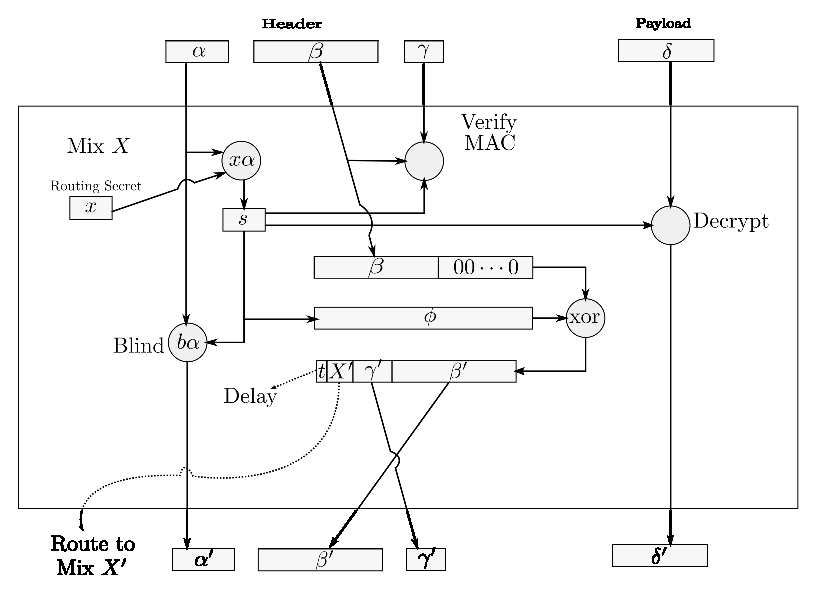
\includegraphics{sphinx1.eps}
  \end{center}
  \caption{The Sphinx packet format (reproduced from~\cite{Sphinx}).}
  \label{fig:sphinx}
\end{figure}

A Sphinx packet (Figure~\ref{fig:sphinx}) flows along a client-selected
route $X_1,\ldots,X_n$ where $n$ is less than some small network defined
constant.  A Sphinx packet consists of an elliptic curve point $\alpha$,
a routing header $\beta$ of a fixed length $L$, a single-use reply block
a MAC $\gamma$ that authenticates the contents of $\beta$, and a body
$\delta$.  Both $\beta$ and $\delta$ are onion encrypted, but $\beta$
uses a stream cipher, while $\delta$ uses a wide block cipher since
it is not authenticated.

Each hop $X$ processes $(\alpha,\beta,\gamma,\delta)$ as follows.  
First, it computes a shared secret $s = x \alpha$ to
derive a replay code, a MAC key, a stream cipher key, 
 a blinding key $b$, and a wide block cipher key. 
It uses the MAC key to check the MAC of $\beta$ and
 then checks its database for the replay code.
It aborts and drops the packet if either the MAC check fails or
 if the replay code is present.  Otherwise it adds the replay code
 to its database.
Next, it pads $\beta$ with $l$ zeros and decrypts the result
 using the stream cipher to produce a $\hat\beta$.
An initial segment of $\hat\beta$ of length $l' < l$ must contain
a valid routing command.  

We discuss some new routing commands in this paper, but the typical
routing command states the next hop $N'$ to which to forward the
packet, and the $\gamma'$ the next hop $N'$ requires. 
In this case, our hop $N$ computes $\alpha' := b \alpha$,
extracts $\beta' := \hat\beta[l'..L+l']$, and
decrypts $\delta$ using the wide block cipher to produce $\delta'$.
Now the packet $(\alpha',\beta',\gamma',\delta')$ is forwarded to $N'$,
 according to whatever mixing rules the protocol specifies.


\subsection{Cross over points}\label{subsec:crossover}

% FIXME: needs a diagram ;-).

A classical mix node command tells the mix to act as a ``cross over''
point by replacing the Sphinx header with a SURB stored in the packet.
We expect the recipient had previously supplied this SURB to the
sender, along with information like the cross over point from which
the SURB works, so this gives the recipient control over routing, 
and provides them with anonymity, even from the sender.  
The sender selects the path to the cross over point, so they can be
anonymous too, even from the recipient.
% TODO: Citation for cross over points?

A {\tt cross over} command provides a length $k$ along with new
 $\alpha''$ and $\gamma''$ that replace our old ones. 
We replace $\beta$ with $\beta'' := \beta'[0..k]$, or equivalently
$\hat\beta[l'..l'+k]$, followed by $L-k$ zero bytes.
\[ \beta'' :=  \beta'[0..k] \,||\, 0\cdots0 \]
In addition, $\delta$ is replaced by the decrypted $\delta'$, 
Now the mix reruns the Sphinx decoding process on the new packet
$(\alpha'',\beta'',\gamma'',\delta')$. 
After this second run there is nothing about the packet that 
identifies it --- not even to the original sender.
We zero the trailing $L-k$ bytes of $\beta''$ before decoding so that
the recipient can compute the required MACs, including $\gamma''$.

As stated, our recipient has chosen the cross over point $X$,
supplied the sender with $(X,\alpha'',\beta'[0..k],\gamma'')$,
and the sender built a route to $X$.  We imagine $\alpha$ to be
twice the size of $\gamma$ and $\gamma$ to be roughly the length of
$X$, so the {\tt cross over} command itself consumes 1.5 hops of $\beta$.
As the recipient picked $X$, this reduces the sender's maximum route
length by roughly 2.5 hops, plus any hops in $\beta''$.
We must bound the length $k$ or else the recipient could prevent
the sender from adding enough hops themselves, what we call a
long SURB attack.

\smallskip 

We could increase the total route length by one if we added a next
hop $X''$ to the {\tt cross over} command, built the tail of $\beta''$
using a stream cipher and sent $(\alpha'',\beta'',\gamma'',\delta')$
to $X''$. We consider this is wasteful because hops cost vastly more
than a few bytes in the header.

Worse, we observe that $\delta'$ has been stripped of all onion
encryption layers created by the sender because the sender must not
know anything about the packet after the cross over point,
 including wide block cipher keys.
We therefore forbid $\delta'$ from being the plaintext message itself
and insist that it be protected with another layer of end-to-end
encryption.  Indeed, this end-to-end encryption layer must use
different ephemeral keys to prevent cross over points from performing
correlation attacks on $\delta'$.

If all SURBs are supplied to the sender by the recipient, then
we could simply provide an extra wide block cipher key with which
the sender pre-encrypts $\delta$ before applying its own onion layers.
We do not assume this because SURBs have a limited lifespan though.  
If the sender does not posses any SURBs, then they could contact the
recipient through a {\em contact point}, and ask for SURB. 
These contact points would act like cross over points, except
that they would supply the SURB themselves from a stash supplied by
the recipient.

In this scenario, it impacts our mix networks' security less if
$\delta'$ is only ever seen by the cross over point, thereby
simplifying our overall design.   In particular, we might not mind
if the cross over point observes an ephemeral elliptic curve point
in $\delta'$, but even tools like Elligator~\cite{elligator} do not
conceal this point from a second hop.

In short, if we added this second hop $X''$ to lengthen the route
then $X''$ might discover its position as the hop after a cross over
point.  We could have a more oblivious hop at the cost of adding a
few bytes to the header.

\smallskip

There are two alternative approaches to encoding the SURB in the 
packet:  

First, the SURB could be placed into a special segment called
$\epsilon$, thus avoiding the long SURB attack check.
We must now however MAC $\epsilon$ like $\beta$ or else any
node in the sender's route can ``tag'' a message allowing its
identification by the cross over point $X$.  We also zero
$\epsilon$ at the cross over point like we zero the trailing
$L-k$ bytes of $\beta''$ currently.  We think placing the SURB
into $\beta$ buys us greater flexibility since $\epsilon$ has become
functionally equivalent to more $\beta$.

Second, we could place the SURB into a prefix of $\delta'$ because,
as noted above, $\delta'$ has been stripped of all onion encryption
layers created by the sender.  In this approach, a packet supports
a slightly larger payload if it does not use a SURB and perhaps
multiple SURBs for multiple recipients, so called garlic encryption.
In the short term, we fear that exploiting these options complicates
our API however.  Also, this scheme complicates the layering of
message and mix encryption.  We shall leave the door open for this
approach in future though becuase suport for multiple SURBs remains
an interesting option.


% \subsection{Sphinx packet construction}

% TODO: briefly explain packet construction ...



% Xolotl-3-mailboxes.tex

\section{Mailboxes}

As mentioned in the introduction, we must never assume that users,
nor any agent they control, is reliably online.  
% ``It's an asynchronous world.''  - Moxie Marlinspike
% https://github.com/WhisperSystems/Signal-Android/blob/master/CONTRIBUTING.md
As a consequence, we must retain messages for an offline recipient
until their client requests delivery.  
At present, there are no successful secure messaging protocols
without this IMAP/POP-like {\em request-and-forward} functionality,
except arguably off-the-record messaging. 


\subsection{Aggregation points}

We expect this necessitates that messages destined for the same
recipient flow into mailboxes at a small number of {\em aggregation
points} that process delivery requests.  These aggregation points 
should learn as little as possible about recipients or senders, but
the recipient should learn the sender's identity from the protocol.
In~\cite{agl-pond-hmac}, Adam Langley explains that Pond has similar
requirements and indicates important advantages of delivery tokens
over more complex schemes, like group signatures~\cite{VLR,BBS}.

We can easily add a ``deliver to mailbox'' command to Sphinx so that
SURBs can act as a delivery token.  In fact, SURBs provide near
perfect delivery properties in sense of~\cite{warner-delivery}.
An aggregation point cannot contribute any knowledge about sender
even when colluding with the cross over point and recipient.
In addition, our SURB hides both the aggregation points and the
mailbox from the sender, which simplifies the recipient's task if
they change aggregation points and mailbox identifiers.

However, we must address a hiccup in how SURBs identify themselves
and senders.

\subsection{Unwinding SURB onion layers}

We noted that a cross over point sees the body, denoted $\delta'$
above, without any wide block cipher encryption layers.  We have
chosen our wide block cipher so that its encryption and decryption
operations provide exactly the same security guarantees and can
safely be swapped.  This conceptual swap happens at our cross over
point so that subsequent hops do not recognize themselves as being
after a cross over point.  They happily apply the decryption
operation without realizing that it further encrypts the body.
However, our recipient must somehow {\em unwind} these layers of
onion encryption, and to do so efficiently the recipient must have
a way to identify which of its SURBs was used, so that they
can select the correct set of keys.

\begin{issue}
How should recipients reconstruct the key materials needed to
unwind the encryption applied by nodes along their SURB's route?
\end{issue}

There are two basic schemes for obtaining the key material to
unwind the encryption applied to $\delta$ from mixes encrypting
during the SURB hops:

First, the recipient may {\em record} the wide block cipher keys used
under a {\it SURB name}.  Any packets at any hop has a natural SURB
name $\eta$ derived from the shared secret $s$.  As an optimization,
we could treat the arriving packet's $\alpha$ as the SURB name at
clients who expect themselves to be recipients.  Any SURB name scheme
has advantages in that it requires no additional space in the header
and provides simple authentication for arriving SURBs.  

Second, our recipient could construct their SURB using a {\em seed}
that they also encode into the ``bottom'' of the SURB itself, so
that they may {\em reconstruct} the original SURB and its keys.
There are potential advantages to encoding a seed in multi-device
scenarios where all devices of a user can decrypt messages without
further communication after sharing some initial key material.

However, to reconstruct the SURB from a seed in an evolving mix
network requires that recipients learn the packet's route, which
requires either that the route be encoded with the seed, which takes
considerable space, or else that the client can identify their view
of the mix network somehow.  If the network itself does not provide
a global consensus like Tor, then multi-device schemes become
extremely difficult.

At present, we believe both schemes to be worth supporting because
they cover fairly distinct use cases, including unusual situations
like in \S\ref{subsec:LEAP}.

In either scenario, our packet takes a predetermined route to the
recipient who unwinds the layers of encryption applied to the body
using information present on their disk and either the packet's alpha
$\alpha$, the shared secret $s$, or their $\beta'$.  

%TODO: Should this be said?
% Mixes delay messages along this route, but so far our recipient cannot change the route. 

\subsection{Redirecting messages}

We want SURBs to be used to reach the aggregation point because
this supports good delivery properties.  We also require the
aggregation point not learn anything about either the sender, or
the route used to reach the aggregation point.  We now turn our
attention to protecting the recipient from their own aggregation
points.

\begin{issue}
How should recipients fetch messages from their aggregation points?
\end{issue}

In principle, recipients could simply send the aggregation point
a packet with a flush mailbox command that launched all pending
packets along whatever remained of their route.  We foresee many
difficulties with such an approach, including simple route length
constraints and packet loss due to network churn, mix node key
lifetime, and clients changing guard nodes, any of which can cause
paths used in SURBs to become unavailable.

Instead, we propose that SURB directed messages should arrive at
an aggregation point without further routing commands.
The aggregation point then stores the incoming SURB's name $\eta$
derived from $s$ along with $\delta'$ in the user's mailbox.

We therefore need a method for our final recipient to retrieve both
$\delta'$ and the corresponding SURB name $\eta$ from her aggregation
point together. 

\subsection{SURB logs}\label{subsec:surb_logs}

We do not consider private information retrieval (PIR)
schemes~\cite{pir} because they increase complexity, invoke disparate
security properties, leak metadata through excessive bandwidth, and do
not support message deletion.
% FIXME: citations needed...

\begin{issue}
How can we send both $\delta$ and $\eta$ through the mix network?
\end{issue}

There is no way to ``squeeze'' our incoming SURB name $\eta_0$ into
the body $\delta$ because the body was previously encrypted with a
wide block cipher and thus cannot be shrunk.

Our recipient could ask the aggregation point to report the waiting
messages, and then send it separate SURBs assigned to each reported
SURB name.  We think this approach could work if the latency were
reasonably low, but the extra round trip creates a problem in a
protocol with even moderate latency. 

Instead, we propose adding a {\it SURB log} $\zeta$ to the header.
Any regular Sphinx hop encrypts $\zeta$ with more of the stream
cipher, but does not include it when verifying the MAC $\gamma$.
An aggregation point that receives fresh SURBs for a nonempty
mailbox simply places the previous SURB name $\eta_0$ into $\zeta$,
places $\delta'$ into the body, and populates the remaining fields
as usual.

For our recipient, there is an incoming SURB name $\eta_1$ that 
controls unwinding back to the state seen by the aggregation point.
We unwind $\zeta$ as well so that our recipient learns $\eta_0$ too,
and may continue unwinding back to the cross over point.
% FIXME: Pictures, please!

We do not MAC $\zeta$, so any adversary can flip bits arbitrarily
there.  As $\eta$ is uniformly random, we can easily make it large
enough to make brute forced search impossible.  An aggregation point
does however witness well-formed $\zeta$ from its incoming packets,
so an aggregation point could identify a message as coming form an
incorrect original sender.

For this reason, one should consider the mix network's sender
identification as an unauthenticated hint that simplifies proper
authentication in the body, say by supporting Axolotl header
encryption.  

We weakly authenticate the $\eta_0$ extracted from $\zeta$,
as being supplied by the aggregation point, because only the client
knows $\eta_1$, and all the layers of encryption applied to $\eta_0$.  
We imagine this weak authentication may help identify the source of
unwanted messages, or a denial of service attack, say by a malicious
contact point.


\subsection{Deletion policy}

To maximize the chance of delivery and to possibly support the user
accessing their messages from multiple devices, aggregation points
should not delete messages until they either need to reclaim the
storage space or are explicitly told to do so by the recipient.

\begin{issue}
After sending a message for final delivery, how should aggregation
points decide to resend or delete the messages?
\end{issue}

In a low latency Stop-and-Go mix, an aggregation points could be
given time-outs after which time it may retry messages which it sent
but for which it never received deletion instructions.

In the high latency scenario though, an aggregation points should
probably  avoid wasting two SURBs from the same batch on the same
message.  A message delivering a subsequent batch can then request
their deletion to avoid re-delivery.


\subsection{Unwinding guards and repeated retargeting}

In Tor, clients rotate circuits every 10 minutes, while holding
fixed their first hop, called a guard node.  This protects clients
from attackers seeking to push them onto a malicious guard
node~\cite{tor-guards}.

In a mix network, packets take much longer routes than tor cells.
There are nevertheless several reasons clients might concentrate
their traffic through a few guard nodes.  In principle, these
guard nodes might even be service providers who know the client. 
In this vein, mobile devices reduce their bandwidth usage and save
battery life by consolidating their messages through notification
servers, so mix clients running on a mobile device might do this as well.
% TODO: Any referenced on batching or other advantages?

At the same time, an aggregation point could hoard a user's messages
until the user selects a malicious guard, so users may wish to avoid
rotating guards too much.  

As a result, any recipient's guard node become a de-facto aggregation
point in that they should hold message for users who will reconnect.
Instead of a mailbox, the SURB should identify the final hop to the
client.  If a user does change the guard, then SURBs used to poll
messages from aggregation points may abandon messages waiting at the
old guard, and this may be common if the mix network has high latency.

We have noted that aggregation points need not delete messages until
told to do so.  Yet, we also envision conversing clients achieving
lower latency by sharing SURBs that arrive directly without passing
through long-term storage aggregation points.  Any such messages
could more easily be left waiting at an old guard.

\begin{issue}
What happens to messages left waiting at a guard instead of an
aggregation point?
\end{issue}

First, we can pick up messages from a guard similarly to how we pick
up message from an aggregation point by extending our SURB unwinding
process. If we require unwinding to support several retargeting
operations, then we simply allow several SURB names in $\zeta$,
 shift $\zeta$ rightward when adding a SURB name $\eta$, and
 shift $\zeta$ leftward when extracting a SURB name during unwinding.

In this scheme, we might notify our previous guard when we
eventually reconnect to the mix network, which leaks information.
We could avoid this by giving our guard some SURBs to message a
mailbox, probably when we first connect.  In this scheme, we might
store three SURB names in the final $\zeta$ for a message that was
meant to be direct.  We would store four for messages that already
passed through a mailbox.

% FIXME: Pictures, please! Especially for the iterative retargeting!
% Having a picture of the complete package format with the
% multi-\eta \zeta in a network diagram that shows an old
% guard, a new guard, a crossover and at least one (storage)
% aggregator (not in this order ;)) would be good.

Second, these concerns about notifying the guard present another
perhaps simpler solution.  We could modify the SURBs given directly
to our contacts to contain a new {\tt deliver} command which acts
like a conditional destination version of our usual {\tt transmit}
command.  A {\tt deliver} command attempts to send the message to
the user, like a {\tt transmit} command, but if it fails for too long
then it attempts to send the message to another mix node, again like
a {\tt transmit} command.  We prepare the remainder of the SURB after
the guard to eventually reach an aggregation point, where the user
may retrieve their message later.

Our second approach imposes only minor complexity on the guard node
processing, while dramatically simplifying the client's interactions
with the mix network.  Anonymity could be impacted by this choice,
albeit in minor ways.
%
In our first scheme, the guard node could possibly uses the SURBs
supplied by the user to help discover the user's aggregation point,
which sounds like a distant threat.  
%
In the our second scheme, we consume header space by using longer
SURBs throughout, or risk leaking that the SURB will attempt direct
dilevery to the cross over point.

We tentatively recommend the second simpler approach, but add support
for extended unwinding to our library regardless.



% Xolotl-3-addresses.tex

\section{Addresses}

...


\subsection{Contact points}

We stated in \S\ref{subsec:crossover} that SURBs might be supplied
by either the sender or the cross over point itself.  We refer to 
a cross over point that supplies the SURB as a {\em contact point}.
We divide contact points acording to the issues they address,
as determined by how they authorize the sender,

We observed in \S\ref{subsec:challenges}, and shall discuss more in
the next section, that mix node keys must rotate for forward secrecy,
but that doing so limits SURB lifetimes.  As a result, clients would
only posses SURBs for contacts they have corresponded with recently.
We cannot even propose that clients message all their contacts within
each key epoch clients may go offline for extended periods.

Instead, we need contact points that restrict the senders to existing
contacts of the recipient.  Recipients can simply inform all their
senders about these contact points and keep the supply of SURBs held
by those contact points updated.  These contact points require
authentication credentials to be provided in the command they extract
from $\beta$.  Recipients must communicate the authentication
credentials required by their contact points to their senders of course.
We note that recipients should still provide senders with SURBs so
that frequent senders do not exaust the SURBs held by contact points,
as well as for faster communications with frequent contacts.

We could deploy many different authentication credentials ranging 
from single-use tokens as in \cite{agl-pond-hmac}, or
 group signatures~\cite{BBS,VLR}, to a simple shared secret.

We think VLR group signatures \cite{VLR} provide an interesting
option for two reasons.  Firstly, SURBs already provide a single-use
token scheme, so a multi-use scheme complements them nicely.  
Secondly, distinct group member private keys could be printed onto
ordinary buisness cards in advance and even the initial message
identifies the card carrying that member privte key.  Identities
can be assigned to these keys after communication is established.  
Importantly sendrs can be revoked without invalidating all existing
keys.  We expect VLR group signatures incur notable computational
overhead for the contact point.  % Worse, this cost grows as more
% senders get revoked and revokations are surprisingly frequent in
% practice \cite{agl-pond-hmac}.
% TODO: Verify that VLR groups signatures scale badly in revokations

As a rule, contact points are an extremely low bandwidth channel
since their stuply of SURBs can easily be exausted.  We must not
reveal any identifying information about the sender to the contact 
point itself during authentication, but authentication should ideally
reveal some $\iota$ to the contact point from which the recipient
can identify the sender.  VLR group signatures and single-use tokens
provide this $\iota$, but a simple shared secret fails to.  We must
now communicate $\iota$ from the contact point to the recipient. 
We could encode $\iota$ into the SURB log, or even empty space in
$\delta$, but this poses two minor problems: 
 Another hop could corrupt $\iota$ masking the true sender.
 Also $\iota$ is large for VLR group signatures.  
%TODO: Verify that $\iota$ is large for VLR group signatures.
We could accumulate a log of $\iota$s on the contact point and send
this log to the recipient when few SURBs reman, but this only
provides verification after the fact.

%TODO: Talk about if we're implementing VLR group signatures?
%TODO: Explain why we cannot simply move the contact points under DoS.


\subsection{New contacts}

We do want special contact points called {\em greeting points} that
do not restrict senders to existing contacts.  A priori, these sound
vulnerable to denal-of-service attacks, and might suffer from SPAM.
We hope that simply moving the advertised greeting points frequently
works, so long as existing contacts never need them thanks to other
contact points.

We need a facility for users to indroduce other users to one another.
because doing so seems essental for group communication.  If Alice 
knows both Bob and Carol then Alice can introduce Bob and Carol by
providing each with either a SURB if the introduction should happen
in a timely fashion, or with authentication credentials for each
others' contact points.  

We require that Alice does not compramise her ability to contact
either Bob or Carol by doing the introduction and that Bob and Carol
can each distinguish the others' messages' from Alice. 
Alice can share single-use token from Bob and Carol of course.
In a VLR scheme, Alice creates the dilivery authorization signature
that Bob and Carol must use.
Also, we recall that $\delta$ must be encrypted at the cross over
point, so Alice can supply Bob and Carol with authentication tokens 
that must live inside $\delta$ and that require verification before
fully decrypting $\delta$.  

% TODO: How much do we wish to explain here? 
% TODO: Our TOFU protocol even?  \cite{tofu} 


\subsection{Provider guards}

We have broadly focussed on strong anonymity properties 





% Xolotl-5-retries.tex

\section{Reliability}

We must ensure reliable message delivery even when some mix nodes
become unavailable.  We should assess nodes' reliability before
publishing their new routing keys, so that more reliable nodes can
be placed into more critical network strata, especially the
aggregation points.

There are however techniques that help address aggregation points
becoming unavailable, like senders sending duplicate messages,
 or aggregation points must mirror one another.
We view mirroring as an interesting approach, but feel it goes far
beyond the scope of our current project, as mirroring well might
entail reencryption.  Also, duplicate messages help reliability
throughout the network.


\subsection{ACKs}

...


\subsection{Duplicate messages}

...
%TODO: Anonymity costs of duplicate messages?
%TODO: Multiple latencies


\subsection{Garlic retries}\label{subsec:garlic_retries}

We cannot necessarily much bandwidth available on the channel
between the client and the mix network.  As an example, Pond
clients support only about 288 messages per day because they
wait on average 5 minutes between messages.

We can reduce the need for duplicate messages on this link if
we tell our cross over point to send them instead, but this requires
providing  it with multiple SURBs so that retries do no violate
replay protection.

In \S\ref{subsec:crossover}, we considered storing SURBs inside
$\delta$, instead of $\beta$, because $\delta$ has no more layers of
onion encryption from Sphinx after a cross over point decrypts it. 
As $\delta$ is large, we may encode several SURBs into $\delta$,
so as to send the same message to multiple recipients, or to send
the same message to the same recipient multiple times.  

In fact, we can achieve this must more easily than sending to
multiple recipients because the recipient can supply several SURBs
with the same cross over point.

These SURBs can have different delays of course, but we can also
provide retries:  Instead of delivery to an aggregation point being
the end of our messages' path, we use a {\tt drop off} command that
delivers the packet to the aggregation point as usual, but also
sends the packet on to yet another hop.  The SURB executing command
routes the packet back to the cross over point, where it executes a
{\tt delete} command that deletes any pending retries.

All this works fine if we use a contact point that supplies holds
SURBs itself, as in \S\ref{subsec:contact_points}, instead of using
a cross over point.  In any case, recipients should supply the SURBs
in groups for {\tt delete} commands to work.

We notes this scheme increases our vulnerability to attacks by the
cross over point:  At best, this {\tt delete} command reveals
dangerous information about what nodes were reachable and that our
message was being sent with redundancy, as opposed to multiple 
recipients.  Also, it assumes the reliability of both the cross over
point and any nodes on the path to it.
%
We shall discuss situations where this may be acceptable in the next section.


\subsection{Email integration}

We have focused on designing an asynchronous messaging architecture
with extremely strong possible privacy properties, including
anonymity for both sender and recipient, even from one another, and
anti-discovery measures for recipients' aggregation points.  
%
We consider this distributed architecture preferable overall, but
we recognize these protections verge on excessive for many users,
that email is tricky to replace, and that email providers may have
benevolent political reasons to remain involved.

We may adopt the {\tt drop off} and {\tt delete} commands described
in \S\ref{subsec:garlic_retries} to integrate our system with email
providers, while giving senders and recipients anonymity from
providers, but not from one another.

We now assume the sender knows both the recipient's aggregation point
and their mailbox name at their aggregation point.  As a result, our
sender may build SURBs to reach the recipient without the recipient
supplying them to either the sender or a contact point.  
In this case, the sender picks the cross over point themselves, 
likely their own Email provider.

In this case, our recipient cannot already know the layers of
encryption applied to $\delta$ after the cross over point.  
We must therefore encode a both a seed and an epoch identifier for
the list of all mix nodes, so that the SURB can be rederived.
This should be included in the {\tt drop off} command and placed into
the SURB log by the recipient's aggregation point.

There is now a risk the recipient's mailbox does not exist. 
In this case, our {\tt drop off} should specify an alteration to
either $\delta$ or the SURB log, and the sender should warn their
cross over point that this alteration means the message was undeliverable.

A priori, there is considerable risk of unwanted messages like SPAM
under this scheme.  As a result, our cross over point $X$, aka the
provider, must require authentication by the sender.  
Recipients must learn the provider when they reconstruct the SURB.  
If they do not, then message decryption necessarily fails.




% Xolotl-5-forwardsec.tex

\section{Key compromises and forward secrecy}\label{sec:forward-sec}

We have observed that high latency anonymity schemes depends upon
nodes using non-ephemeral key material, thus opening them to key
compromise attacks that do not impact onion routers like Tor.
There are several natural ways one might harden mix networks against
node keys being compromised. 


\subsection{Key rotation and replay attacks}

As a rule, mix networks must prevent replay attacks, normally using
a database of some form.  As this database must not grow indefinitely,
mix nodes must rotate their keys periodically.  These keys should be
destroyed when no longer used to provide a measure of forward security.

In principle, we could rotate keys quickly so that the compromise
window for each key stays short.  However, we must also support
single-use reply blocks (SURBs) so that anonymous users can receive
messages.  As SURBs are built to a specific set of node keys they
cannot outlive the key rotation schedule.  This creates a tension
between forward security and usability.

We could rotate node keys slow enough for our usability goals, but add
a faster rotating identity-based epoch key issued by a collective of
trusted nodes, and deform the SURB's key material to account for this
rotating identity-based epoch key.
% FIXME: citation needed (I assume somebody published this atrocity?)
This buys use forward security, assuming at least some trusted node
does not get compromised, but would be difficult to deploy in practice.

We could use punctured encryption~\cite{libforwardsec} for our
mix nodes key, so that mix nodes who correctly puncture their key
after decrypting a message cannot decrypt the same message again. 
% TODO: Cite an older article on punctured encryption.
As a rule, punctured encryption schemes require $O(n)$ time for
decryption where $n$ is the number of punctures so far.  

There are techniques for epoch based puncturing that make $n$ less
than the number of packets.  In a mix network, these are either
equivelent to shortening node key lifetimes, or else require
deforming SURBs.  Any scheme for deforming SURBs requires a delicate
proof of security because mix network packet formats based on more
malleable key material tends to be broken~\cite{Danezis2006}. 
Also, these ideas all require slower pairing-based cryptography that
would increase our mix node's vulnerability to denial of service attacks. 

After ruling out these solutions, our question remains unresolved : 

\begin{issue}
Is there a forward secrecy mechanism to reduce the risk of mix node
keys being compramized after messages traverse the network?
\end{issue}


\subsection{Post-quantum cryptography}

Along with the primitives being relatively young and poorly explored,
an important obstacle to deploying post-quantum cryptography is
the comparatively large key sizes.  As a comparison: 
%
A recent Ring-LWE key exchange New Hope~\cite[\S7, p.10]{NewHope} needs
 key sizes of 1824 or 2048 bytes, both of which must be ephemeral,
while one McEliece-like system McBits~\cite{McBits,PQ-InitRec}
 needs a staggering 1MB for public keys.
%
Super-singular isogeny Diffie-Hellman (SIDH)~\cite[p. 21]{SIDH-2016} keys
are only 564 bytes, or 751 bytes uncompressed, but
 the key exchange requires at least 100 times as much CPU time as
 an ECDH key exchange with equivalent classical security.

Anonymity tools like mix networks are sensitive to key size because 
users interact with numerous nodes and key material overhead is 
quadratic in the number of hops. % $n(n+1)/2$
% FIXME: Eh, what? How? Where? It is linear!!?!?!?!!

% FIXME: need to add a conclusion from this, i.e
% that we do not want to do PQC on every hop or
% for every message, but might be happy with
% setting up PQC-secured pairwise crypto with
% one designated hop on a path.

\subsection{Sphinx key blinding}

% FIXME: deduplicate with what we had above, most of it is duplicated
% and/or ought to have been said when we first talked about Sphinx.
% After that, this subsection can probably go away.

Sphinx~\cite{Sphinx} is a packet format for anonymizing mix networks
that is provably secure in the universal composability framework, and
 addresses the key material burden by mutating or reblinding a
 single ephemeral public key $\alpha$ with each hop,
 as opposed to unwrapping an unrelated public key for each hop.

In Sphinx, an elliptic curve point is blinded by multiplication with
a shared secret scalar derived from the Diffie-Hellman exchange using
the same point:
After selecting an initial private scalar $x_0$,
 public curve point $\alpha_0 = x_0 G$, and 
 a sequence of $n$ nodes with keys $Y_i = y_i G$,
we recursively define 
\[ \begin{aligned}
\textrm{shared secret}\quad
 s_i &:= x_i Y_i = y_i \alpha_i \mathcomma \\
\textrm{blinding factor}\quad
 b_i &:= H(s_i) \mathcomma \\
\textrm{next private key}\quad
 x_{i+1} &:= b_i x_i \mathcomma \\ % \quad\textrm{and} \\
\textrm{next public key}\quad
 \alpha_{i+1} &:= b_i \alpha_i \quad\textrm{for $i < n$.} \\
\end{aligned} \]
Our $i$th node replaces $\alpha_i$ by $\alpha_{i+1}$.


\subsection{Problems combining post-quantum cryptography and Sphinx}

We ask if any post-quantum public key exchanges admit 
a key blinding operation suitable for Sphinx. 
At present, the answer appears to be {\bf no}, for similar reasons to
why these primitives still lack convenient signature schemes. 
In particular, there are blinding operations but they incur significant
costs  that are asymptotic in the number of hops.

In SIDH, a public key is an isogeny whose kernel consists $p$-torsion
for $p=2$ or $3$.  It reveals guide points in the $5-p$-torsion but
must not reveal the image of any known $p$-torsion points.  
As a result, current attempts to blind SIDH keys for signature schemes
add another torsion prime beyond 2 or 3, increasing the size of the
base field.  In Sphinx, we could invent new shared $p$-torsion guide
points for computing the blinding isogeny, thus avoiding these issues.
We expect SIDH remains quite new and blinding in this way is unheard of,
so doing this reuqires time to build confidence in these operation.  
Worse, there are currently open questions around key validation in
SIDH that prevent using long term keys~\cite{SIDH-NoValidation}, which
Sphinx requires.

In Ring-LWE, there is enough flexibility for blinding constructions
that increase the key size, fully homomorphic encryption schemes that
avoid this increase, and even a primitive similar to universal
reencryption exists~\cite{963628}.  In all cases however, we still
increase key sizes dramatically over existing key exchanges and we face
difficult key wrap problems with the fully homomorphic encryption
schemes.

We consider such schemes currently unsuitable for another reason though: 

In Sphinx, there is no requirement that the blinding keys $b_i$ be
drawn from a uniform distribution because standard assumptions on
elliptic curves suitable for cryptography ask that an adversary has
no appreciable advantage in determining the correspondence between
$\alpha_i$ and $\alpha_{i+1}$ without knowing $b_i$.  
Indeed, the Curve25519 function commonly used for Diffie-Hellman key
exchange in Sphinx implementations goes so far as to set the high bit
of the private scalar as a protection against non-constant time
implementation.
% FIXME: there is a sentence missing here relating this back to
% RLWE, i.e saying that RLWE requires keys selected from uniform
% distribution. ``there are also'' here makes no sense.
% It is totally unclear what algorithms you are talking about!!!
There are also cryptographic algorithms like signatures for which
this assumption does not suffice and blinding scalars must be chosen
from a uniform distribution.

There are similar assumptions underlying both Ring-LWE and SIDH.
We believe these assumptions should be viewed as stronger than simply
assuming the security of the key exchange scheme itself, partially
due to their youth, but also because the underlying operations cannot
so easily yield a uniform distribution on public keys.  We believe
further research into signature schemes might help build our confidence
in blinding operation with Ring-LWE and SIDH, but this will take time.

As these schemes remain young, we want post-quantum public key
systems to be used in a hybrid protocol with an elliptic curve scheme,
so that an adversary must break both.  There is an imminent danger
that blinding operations can fail if only one of the component schemes
fails.

As an example, we consider a Sphinx-like mix net packet format that
employs the ordinary Curve25519 key exchange for blinding along side
a post-quantum scheme with any magical properties we desire.  
A quantum computer can break this by computing $b_{\alpha,\alpha'}$
such that $\alpha' = b_{\alpha,\alpha'} \alpha$ for every pair of
incoming $\alpha$ and outgoing $\alpha'$.  Any $b_{\alpha,\alpha'}$
with high bit zero cannot be correct, thus giving the adversary at
least a 50\% advantage in guessing packet routes correctly.

We can theoretically correct this by using a scalar multiplication that
does not zero the high bit in the scalar.  In doing so, we must keep
the multiplication by the cofactor so that the adversary cannot tag
packets by injecting small subgroup elements that do not impact the
key exchange itself.  These are standard moves in elliptic curve 
cryptography that work since the scalar multiplication is bijective.
To be blunt, the elliptic curve scalar multiplication can act as
a blinding operation in a hybrid protocol because the blinding itself
can be made information theoretically secure.

While this may suffice to secure a hybrid scheme against post-quantum
attacks against the Elliptic curve, we encounter a fatal difficulty
if we imagine that instead our post-quantum key exchange might be
broken while elliptic curves remains secure.  
There are no known blinding operations that provide information
theoretic security, so attacks on the post-quantum component must be
expected to yield an advantage in guessing packet routes.

\begin{issue}
Is there a post-quantum key exhange suitable for usage Sphinx or
another mechanism of introducing post-quantum key material?
\end{issue}

% \subsection{Hybrid schemes using separate keys}

We could build a hybrid protocol if our post-quantum key exchange
used separate keys for each hop instead of blinding.  These keys
could be packaged into $\beta$ along with the routing directions and
MACs for Sphinx, but doing so makes the total size of post-quantum 
key material quadratic in the number of hops, and these post-quantum
keys are already extremely large.
% FIXME: again, how do you get to quadratic!?!?!?!?
In this vein, a circuit based approach like Tor at least avoids
transmitting unnecessary key material, but it exposes circuit
metadata by doing so. 

Instead, we draw inspiration from fs-mixes~\cite{fs-mix}%
\footnote{In fact, we developed Xolotl without knowing about fs-mixes
but the comparison simplifies our exposition.} and the
 Axolotl ratchet~\cite{TextSecure}.
We shall provide some background on these two topics before
addressing the two issues of this section in the next section.


\subsubsection{fs-mixes}
% FIXME: combined text that was previously spread all over
% the document here, but needs editing ...

In fs-mixes~\cite{fs-mix}, a mix node derives a $(k,v)$ from from
each key exchange and records $(k,v)$ in a name-value store. 
We already do something similar for  replay protection, but this
new name-value store outlives our public key rotation schedule. 
A subsequent packet sent in another public key epoch may ask that $v$
be hashed into the key exchange after revealing its name $k$.  

These fs-mixes could be viewed as a form of ``ratchet'' not wholly
unlike off-the-record (OtR) messaging ratchet~\cite{OtR}, sometimes
described as a three-step Diffie-Hellman ratchet.
We shall extend fs-mixes to provide stronger protection and be more
reliable, while retaining their feature of introducing key matierial
not directly derived from the current packet's public key exchange.  
Intuitively this parallels how the Axolotl ratchet extends
OtR with a hash iteration ratchet.

In fs-mixes, every packet leaves a trace of symmetric key materials
$v$ that {\it one} later packet can reference with its name $k$. 
In principle, we could chain these traces similarly to how
off-the-record messaging \cite{OtR} chains key exchanges.
In fact, we could buy ourselves a measure of post-quantum protections
through chaining if our initial trace pairs $(k,v)$ were created with
a post-quantum key exchange.  

Yet, we cannot employ chaining with fs-mixes directly because doing
so magnifies any unreliability in our mix network, as any lost packet
leaves the traces unpredictable by the client. 

\subsubsection{Axolotl}
% Axolotl refresher
\def\ck{\texttt{ck}}
\def\rk{\texttt{rk}}
\def\mk{\texttt{mk}}

The Axolotl ratchet~\cite{TextSecure} replaces the off-the-record
messaging ratchet's three-step process with a two-step procedure
that omits advertising a new key update.  Instead, Axolotl continues
using the same public key $A = a G$ in each packet until witnessing
the other side change their key $B = b G$.  Then, Axolotl does the DH key
exchange between the sender's new public key $A$ and the receiver's
public key $B$ that was last seen by the sender.

As in OtR, there is a {\it root key} $\rk$ that Axolotl advances by
hashing it with the results of the DH key exchange.  Axolotl avoids using the same key for
repeated encryptions when the receiver remains silent by deriving the
{\it chain key} $\ck_i$ for a hash iteration ratchet from the root key.

\[ \begin{aligned}
\textrm{root advance}\quad
r' &:= H(r \,||\, a B) = H(r \,||\, b A) \\ % \mathcomma
\textrm{chain start}\quad
 \ck_0 &:= H(\textrm{``Start''} \,||\, \rk) \\
\textrm{chain advance}\quad
 \ck_{i+1} &:= H(\textrm{``Chain''} \,||\, \ck_i)  \\
\textrm{message keys}\quad
 \mk_{j+1} &:= H(\textrm{``Message''} \,||\, \ck_i)  \\
\end{aligned} \]

These ratchet constructions like Axolotl and OtR remain secure against
Shor's algorithm {\it if} the root key is first instantiated with some
post-quantum key exchange, and is twice the desired security level. 
In this case, the ratchet does not provide any post-quantum forward
security per se, but that might be perfectly acceptable given current
obstacles to building quantum computers, and the large key sizes of
some post-quantum key exchanges. 

Axolotl meshes poorly with the mix networks for two key reasons:
\begin{enumerate}
 \item
 We would prefer to exploit the elliptic curve point
 already in the Sphinx header, which must change with each packet
 to avoid correlation attacks; 
 however, Axolotl must hold its key constant until receiving a response.
 \item
 We cannot make mix nodes to respond to the sender, as that
 be comes an onion routing like scheme and the additional traffic
 would make it much more vulnerable to traffic analysis.
\end{enumerate}


% Xolotl-6-ratchet.tex

\section{The Xolotl ratchet}

\def\cn{\texttt{cn}}
\def\DH{\texttt{DH}}
\def\lk{\texttt{lk}}
\def\sk{\texttt{sk}}
\def\ECDH{\textrm{ECDH}}

We resolve these tensions by ``swapping the order'' of the hash
iteration ratchet and the two-step Diffie-Hellman ratchet that make
up Axolotl, creating what we call the Xolotl ratchet.   

We have no root key per se in the Xolotl ratchet.  
Instead, we have only a hash iteration ratchet, called a branch,
consisting of a {\it chain key} $\ck_j$ representing the head of the
ratchet and {\it link keys} $\lk_j$, which Axolotl called message
keys.  We hash link keys $\lk_j$ with the shared secret $s_i$
derived from the key exchange in Sphinx to produce both an improved
shared secret $t_j$ for another layer of Sphinx and a {\it berry key}
$r_j$.  These berry keys replace the root keys in Axolotl, with the
key difference being that once the client determines the message
passed through the network successfully, it can decide to spawn a new
hash iteration ratchet from a berry key.
Thus, the evolution of the Xolotl ratchet is driven by one party, while
the Axolotl ratchet branches based on actions driven by both parties.

% FIXME: is mid-evil supposed to be cute?
We address a branch with a mid-evil naming convention: A branch's own
proper name has the form $(f,b)$ where $f$ is its family name
determined by its parent branch, and $b$ is the index of the berry
from which it grew.  In essence, we address the branch as ``5th child
of George'', or $(f,b)$, under the assumption that everybody already
knows the great deeds of the branch's parent ``George'', or $f$ for
short.  There is, however, a family name $f'$ assigned to $(f,b)$.
Hence, once $(f,b)$ has performed its own great deed --- that is,
successfully delivered a message where the delivery was confirmed to
the sender --- then the children of $f' = (f,b)$ may be addressed as
$(f',\cdot)$.

\subsection{Birth of a Xolotl ratchet}

PQC.
...


\subsection{Formal Xolotl ratchet description} 

A node begins as if decoding a typical Sphinx packet by
 producing the shared secret $s_i$, verifying the MAC, and 
 unwrapping one layer of the header's onion encrypted $\beta$,
producing a $\beta'$, but then pauses to check for a ratchet command.
If the ratchet command is not found, then our node continues with
Sphinx as usual.  
In particular, it takes $\beta_{i+1}$ to be $\beta'$,
derives the blinding factor $b_i$,
blinds the public key as $\alpha_{i+1} := b_i \alpha_i$,
extracts the next hop $n_{i+1}$ and MAC $\gamma_{i+1}$,
unwraps an onion layer from the body $\delta_i$,
 yielding $\delta_{i+1}$, and queues the new packet
$(\alpha_{i+1},\gamma_{i+1},\beta_{i+1},\delta_{i+1})$ for $n_{i+1}$.

If a ratchet command is found, then we extract the ratchet instructions
instead.  These ratchet instructions consist of a branch address,
which contains a branch family name $f$ and a berry index $b$,
 as well as a chain index $j'$,
along with an intermediate MAC $\gamma'$.
% perhaps along with information for closing the previous chain. 

If the branch $(f,b)$ is unknown, then we locate its parent's
proper name $(f_p,b_p)$ using $f$ alone, and extract the berry
key $r$ with berry index $b$ on $(f_p,b_p)$,
 aborting if $f$ or berry $b$ on $(f_p,b_p)$ do not exist.
From $r$, we define
\[ \begin{aligned}
\textrm{family name}\quad
 f' &:= H(\textrm{``Family''} \,||\, r) \quad\textrm{and} \\ % \mathcomma \\
\textrm{chain start}\quad
 \ck_0 &:= H(\textrm{``Start''} \,||\, r) \mathperiod \\
\end{aligned} \]
On our branch $(f,b)$, we inductively define 
\[ \begin{aligned}
\textrm{chain keys}\quad
 \ck_{j+1} &:= H(\textrm{``Chain''} \,||\, \ck_j) \quad\textrm{and} \\ % \mathcomma \\
\textrm{link keys}\quad
 \lk_j &:= H(\textrm{``Link''} \,||\, \ck_j) \mathperiod \\
\end{aligned} \]
In advancing the chain to index $j'$, we save any 
intermediate $\lk_j$ for later use by out of sequence packets.

We now have the particular $\lk_{j'}$ requested by our ratchet 
instructions $(f,b,j')$, so we may define 
\[ \begin{aligned}
\textrm{packet keys}\quad 
 s' &:= H(\lk_j \,||\, s_i) \quad\textrm{and} \\ % \mathcomma \\
\textrm{berry keys}\quad 
 r' &:= H(\textrm{``Berry''} \,||\, s') \mathperiod \\
\end{aligned} \]
We first replace $s_i$ by $s'$ in our Sphinx-like component
and verify the intermediate MAC $\gamma'$.  If this verification
fails, then we abort and abandon our ratchet database transaction.
We thus assume the verification succeeds.  

We now save $r'$ as the berry key for $(f,b,j')$, and commit any
other ratchet database changes, including erasing $r$ or any 
$\ck_i$ previously recorded.  Our branch $(f,b)$ has started
earning the short name its children will use.  
Also, our Sphinx-like component continues, but now using $s'$.
To be specific, it derives the blinding factor $b_i$,
blinds the public key as $\alpha_{i+1} = b_i \alpha_i$,
unwraps a second layer of $\beta$ to extracts the
 next hop $n_{i+1}$ and MAC $\gamma_{i+1}$ and 
 producing our $\beta_{i+1}$,
unwraps an onion layer from the body $\delta_i$,
 yielding $\delta_{i+1}$, and queues the new packet
$(\alpha_{i+1},\gamma_{i+1},\beta_{i+1},\delta_{i+1})$ for $n_{i+1}$.

 \begin{figure}[b!]%[h!]
   \begin{center}
\begin{tikzcd}[ampersand replacement=\&, column sep=small]
\cdot \ar[r] \& \cdot \ar[r] \ar[d] \& \cdot \ar[r] \ar[d] \& \cdot \ar[r] \ar[d] \& \ck \ar[r, dotted] \& ? \& \\
 \& \lk \ar[d] \& \lk \ar[d]  \& \lk \ar[d] \&  \& \& \\ 
 \& \ECDH \ar[d] \& \ECDH \ar[d] \& \ECDH\ar[d] \&  \& \& \\
 \& r \& r \ar[dddll, in=90, out=270] \& r \ar[dddlll, dotted, in=30, out=270] \&  \& \& \\
\\
\\
\cdot \ar[r] \& \cdot \ar[r] \ar[d] \& \cdot \ar[r] \ar[d] \& \cdot \ar[r] \ar[d] \& \cdot \ar[r] \ar[d] \& \ck \& \& \\
 \& \lk \ar[d] \& \lk \ar[d] \& \lk \ar[d, dotted] \& \lk \ar[d] \&  \& \& \\ 
 \& \ECDH \ar[d] \& \ECDH \ar[d] \& ? \& \ECDH\ar[d] \&  \& \& \\
 \& r \& r \&  \& r \&  \& \& \\
\end{tikzcd}
% FIXME: ECDH should probably be SPHINX+? 
\end{center}
\end{figure}


\subsection{Faster chains}

We have described a simple linear hash iteration ratchet above.  
These work well in Axolotl because the sender controls the desired
order of delivery and the transport makes some effort to comply.

In Xolotl, we envision using ratchets when receiving a message 
using a single-use reply blocks (SURBs), as well as when sending.
We should expect SURBs to be used in a far more haphazard way or
indeed discarded when node keys rotate.  

Axolotl also benefits from being used between established contacts,
while mix nodes would provide Xolotl ratchets as a service, likely
for free.  We therefore worry malicious clients might ask mix nodes
to forward ratchets for extreme distances as a denial of service
attack, while the mix node cannot easily distinguish this malicious
behavior from poor SURB usage.

We address these concerns by optimizing our procedure for advancing
the chain key.  We reserve the low $l$ bits of the chain index
for a chain key that works as described above.  
If our index $j$ has a nonzero bit among its lower $l$ bits,
meaning $j \& (2^l-1) \neq 0$, then
we define
\[ \begin{aligned}
 \ck_{j+1} &:= H(\textrm{``Chain''} \,||\, \ck_j) \quad\textrm{and} \\ % \mathcomma \\
\end{aligned} \]
We reserve bit $l$ and higher for a faster tree-like {\it train key}
built using heap addressing.  If the lower $l$ bits of $j$ are
all zero, meaning $j \& (2^l-1) \neq 0$, then we define 
\[ \begin{aligned}
% \textrm{train left}\quad
 \ck_{2j} &:= H(\textrm{``Left''} \,||\, \ck_j) \mathcomma \\
% \textrm{train right}\quad
 \ck_{2j+2^l} &:= H(\textrm{``Right''} \,||\, \ck_j) \mathcomma \\
% \textrm{chain key}\quad
 \ck_{j+1} &:= H(\textrm{``Chain''} \,||\, \ck_j) \quad\textrm{and} \\
\end{aligned} \]
In both case, we could define the link key $\lk_j$ as before, but
the actual key derivations functions could differ between these two
cases, and doing so appears more efficient.


\subsection{State of a Xolotl ratchet}

What are the various maps a xolotl router needs to keep?
$f' \to (f,b)$, $(f,b) \to (j,ck_j,lk_j)$,
$(f,b,i) \to lk_i$ for $i < j$ if message not received;
left/right/train key data structure modifications.

...


\subsection{Expiration of a Xolotl ratchet}

When is which key discarded.  Be precise.

For example, I do not think we need to keep $(f,b)$ if
$f'$ has been used, but we did NOT talk about
how the message involving $f'$ tells us about
the maximum $j$ for which we need to keep
$(f,b) \to (j,ck_j,lk_j)$.

I don't even see an explicit statement that we
cannot fork two berries of the same $f'$ into ratchets...




\subsection{Analysis}

We take $r$ to be 256 bits so that, assuming the initial ratchet
source was created using a post-quantum key exchange, then our
Xolotl ratchet provides 128 bits of post-quantum security.

In addition, Xolotl provides a measure of forward secrecy against
a classical adversary in that the symmetric key information $r$,
$\ck_j$ for $j<j'$, $\lk_{j'}$, and $s'$ all gets erased when
the packet gets queued.  An adversary who later compromises the
private key of our node $n_i$ learns the next hop only for packets
that did not employ any ratchet at $n_i$.

For these advantages, we have exposed,
 to the node $n_i$ hosting the ratchet, that all packets using this
particular ratchet were directed by the same party, making that
party either the sender or receiver if the packet is a SURB.

We expect Xolotl ratchets to be more reliable than fs-mixes because
the hash iteration ratchet component permits ratchet reuse even when
packets get dropped or delayed.  There is a corresponding cost in
that we reveal a connection between far more packets to the node
$n_i$ hosting the ratchet.

There is no need for every hop to employ a ratchet, % though, 
but specific usage patterns require detailed analysis.

\[ \begin{aligned}
\textrm{User} \to &\textrm{Tor} \to \textrm{Xolotl} \to \textrm{Sphinx} \to \\
\quad &\to \textrm{Xolotl} \to \textrm{Sphinx} \to \textrm{Cross} \to \cdots 
\end{aligned} \]

If ratchets are used at only certain hops, then the mix learns
information about its role and position in the route.  
We could mitigate this by consolidating ratchets on specified mix
nodes, presumably with more storage and/or hardened hosting, but
this doing so concentrates our forward secrecy and post-quantum 
defenses as well.

In Tor, there is a more restrictive procedure for selecting the
first hop in a circuit, called a {\it guard} node.  We expect
mix networks will benefit from specialized guard selection as well.
Assuming mix nodes can easily distinguish clients from mix nodes,
there is no need for a ratchet at guard node because the client and
the mix node should use a conventional ephemeral key exchange,
likely a hybrid of an elliptic curve and post-quantum key exchange.

An initial set of ``guard'' ratchets could be created anew for each
session, possibly distinct from the client's actual guard nodes.

We believe that retaining middle ratchets for longer periods could
improve forward secrecy over creating them all anew with each session. 
There are many concerns around this point however, primarily balancing
the improved forward secrecy with the risk of linking packets across
different sessions, but also
 practical matters like ratchet storage requirements on mix nodes.  

Ratchet key material does not expire with node keys.  Indeed, even
berry keys may outlive node keys because the sender simply remembers
them.  We may therefore set ratchet key expiration based upon storage
concerns. 


\section{Implementation}

%TODO: Xolotl in Rust

\subsection{Abuse}

%TODO: Jeff's delay selection system

\subsection{Integration}

%TODO: LEAP and Panoramix project

%TODO: pEp for migration. Lake for storage and messaging.

\begin{figure}
\begin{center}
\begin{tabular}{|c|c|c|} \hline
   MTA & IM & (sensor network protocol) \\ \hline
   \multicolumn{3}{|c|}{{p$\equiv$p}}  \\ \hline
   & \multicolumn{2}{|c|}{{\bf Lake}}   \\ \cline{2-3}
   & \multicolumn{2}{|c|}{{\bf Xolotl}} \\ \cline{2-3}
   \raisebox{1.5ex}{SMTP} & CADET~\cite{cadet} & GNU Name System~\cite{gns}  \\ \cline{2-3}
   & \multicolumn{2}{|c|}{GNUnet-CORE}  \\ \hline
   \multicolumn{3}{|c|}{TCP/IP}       \\ \hline
   \multicolumn{3}{|c|}{Ethernet}     \\ \hline
\end{tabular}
\end{center}
\caption{A plan for replacing IMAP/SMTP with a few extra layers.}
\label{fig:layers}
\end{figure}


\section{Performance evaluation}

Using Bloom filter, how much storage per message?
Give resulting key rotation frequencies for realistic
scenarios. (all calculated)

Bandwidth overhead (ok to do mathematically, but precise,
in bytes).  Computational overhead (measured).

Expected latency by pool strategy. (simulated or calculated)
% We might ignore that and defer to Loopix paper

Messages per second on realistic hardware. (calculated from
microbenchmarks is sufficient)

Required replication level for different reliability assumptions.
Assume different reliabilities for ordinary mixes vs. aggregators
(aggregation points are picked based on known reliability).  How high
does availability need to be to keep replication reasonably low?
(calculated)

Total (system-wide) financial cost per message including reliability
for 99.9999\% availability under realistic assumptions about node
availability. (Assume Amazon EC2 compute node profile for availability
and cost on the one hand, and say a Raspberry Pi at home with typical
DSL-like network (un)availability with Indian-style power outages on
the other)

Discussion on use of Taler to pay for service.
% Riseup/LEAP version viable. 
% Paying aggregation points might be viable. 
% Paying mixes in obnoxious due to overhead. 


\section{Improvements}

We expect that a malicious mix node hosting a Xolotl ratchet learns
that all packets using the ratchet were directed by the same party,
either the sender or receiver.  Considering the modest delay created
by mixes, this allows a weak correlation to be made between ratchet
use and the respective client being online.

A simple counter-measure would be support for a delay mode where
clients can flag messages to be artificially delayed by mixes beyond
the usual delay for mixing.  This could be used to create messages
that traverse the client's ratchet at times where they have been
offline for a while, thereby reducing the correlation between ratchet
use and the client being online.

Another mitigation strategy would be for clients
to share particular ratchet configurations with other nodes.
If several link keys from the same branch can be shared anonymously,
then the sharer risks nothing in doing so, assuming pre-image
resistance for our hash function.  Thus, another way of destroying the
link between ratchet use and user being online would be to share a
batch of link keys from the same branch with a mix node so that it
could utilize our ratchet for messages it needed to send anyways.
However, this assumes mix nodes send numerous messages over the mix
network, which our design currently does not require.

We observe that anyone using this shared link key could gain a berry
key that only they know, along with the mix node hosting the ratchet,
thus allowing them to create a whole new branch.  It follows that,
if individual shared link keys can be retrieved anonymously, then
the recipient of the shared link key risks only that the key fails.
Thus, this creates a minor problem in the form of denial of service
attack against the receiver of such a shared ratchet.

In practice, we cannot provide perfect anonymity in either sharing or
retrieving shared link keys, and retrieving lone link keys sounds
problematic.  Yet, there may be an opportunity here for a second
anonymity system that communicates these shared link keys.
% FIXME: not sure I understand ``lone link keys'' here.


\section*{Acknowledgements}

This work benefits from the financial support of the Brittany Region
(ARED 9178) and a grant from the Renewable Freedom Foundation.
% FIXME: Do you have productive discussions to acknowledge, i.e.
% with George or other pandemix people?

%\newpage

% TODO: Briefly mention Proof-of-onion and \cite{TorPathToTorCoin} 

\bibliographystyle{abbrv}
\bibliography{mix,nonmix,or,msg,pq,rlwe,sidh,gnunet}

\end{document}


\section{}







Anonymous messaging proposals have traditionally either avoided
request-and-forward facilities, due to metadata leakage \cite{??},
or addressed it using private information retrieval (PIR) schemes
\cite{??}.  These PIR schemes increase complexity, invoke disparate
security analysis techniques, and still leak considerable metadata.




